\documentclass[tikz]{standalone}
\usepackage{amsmath}
\usepackage{amssymb}
\usepackage{tikz}
\usepackage{xcolor}
\usepackage{bm}         % For bold math symbols
\usetikzlibrary{arrows.meta} % For better arrow tips

\begin{document}

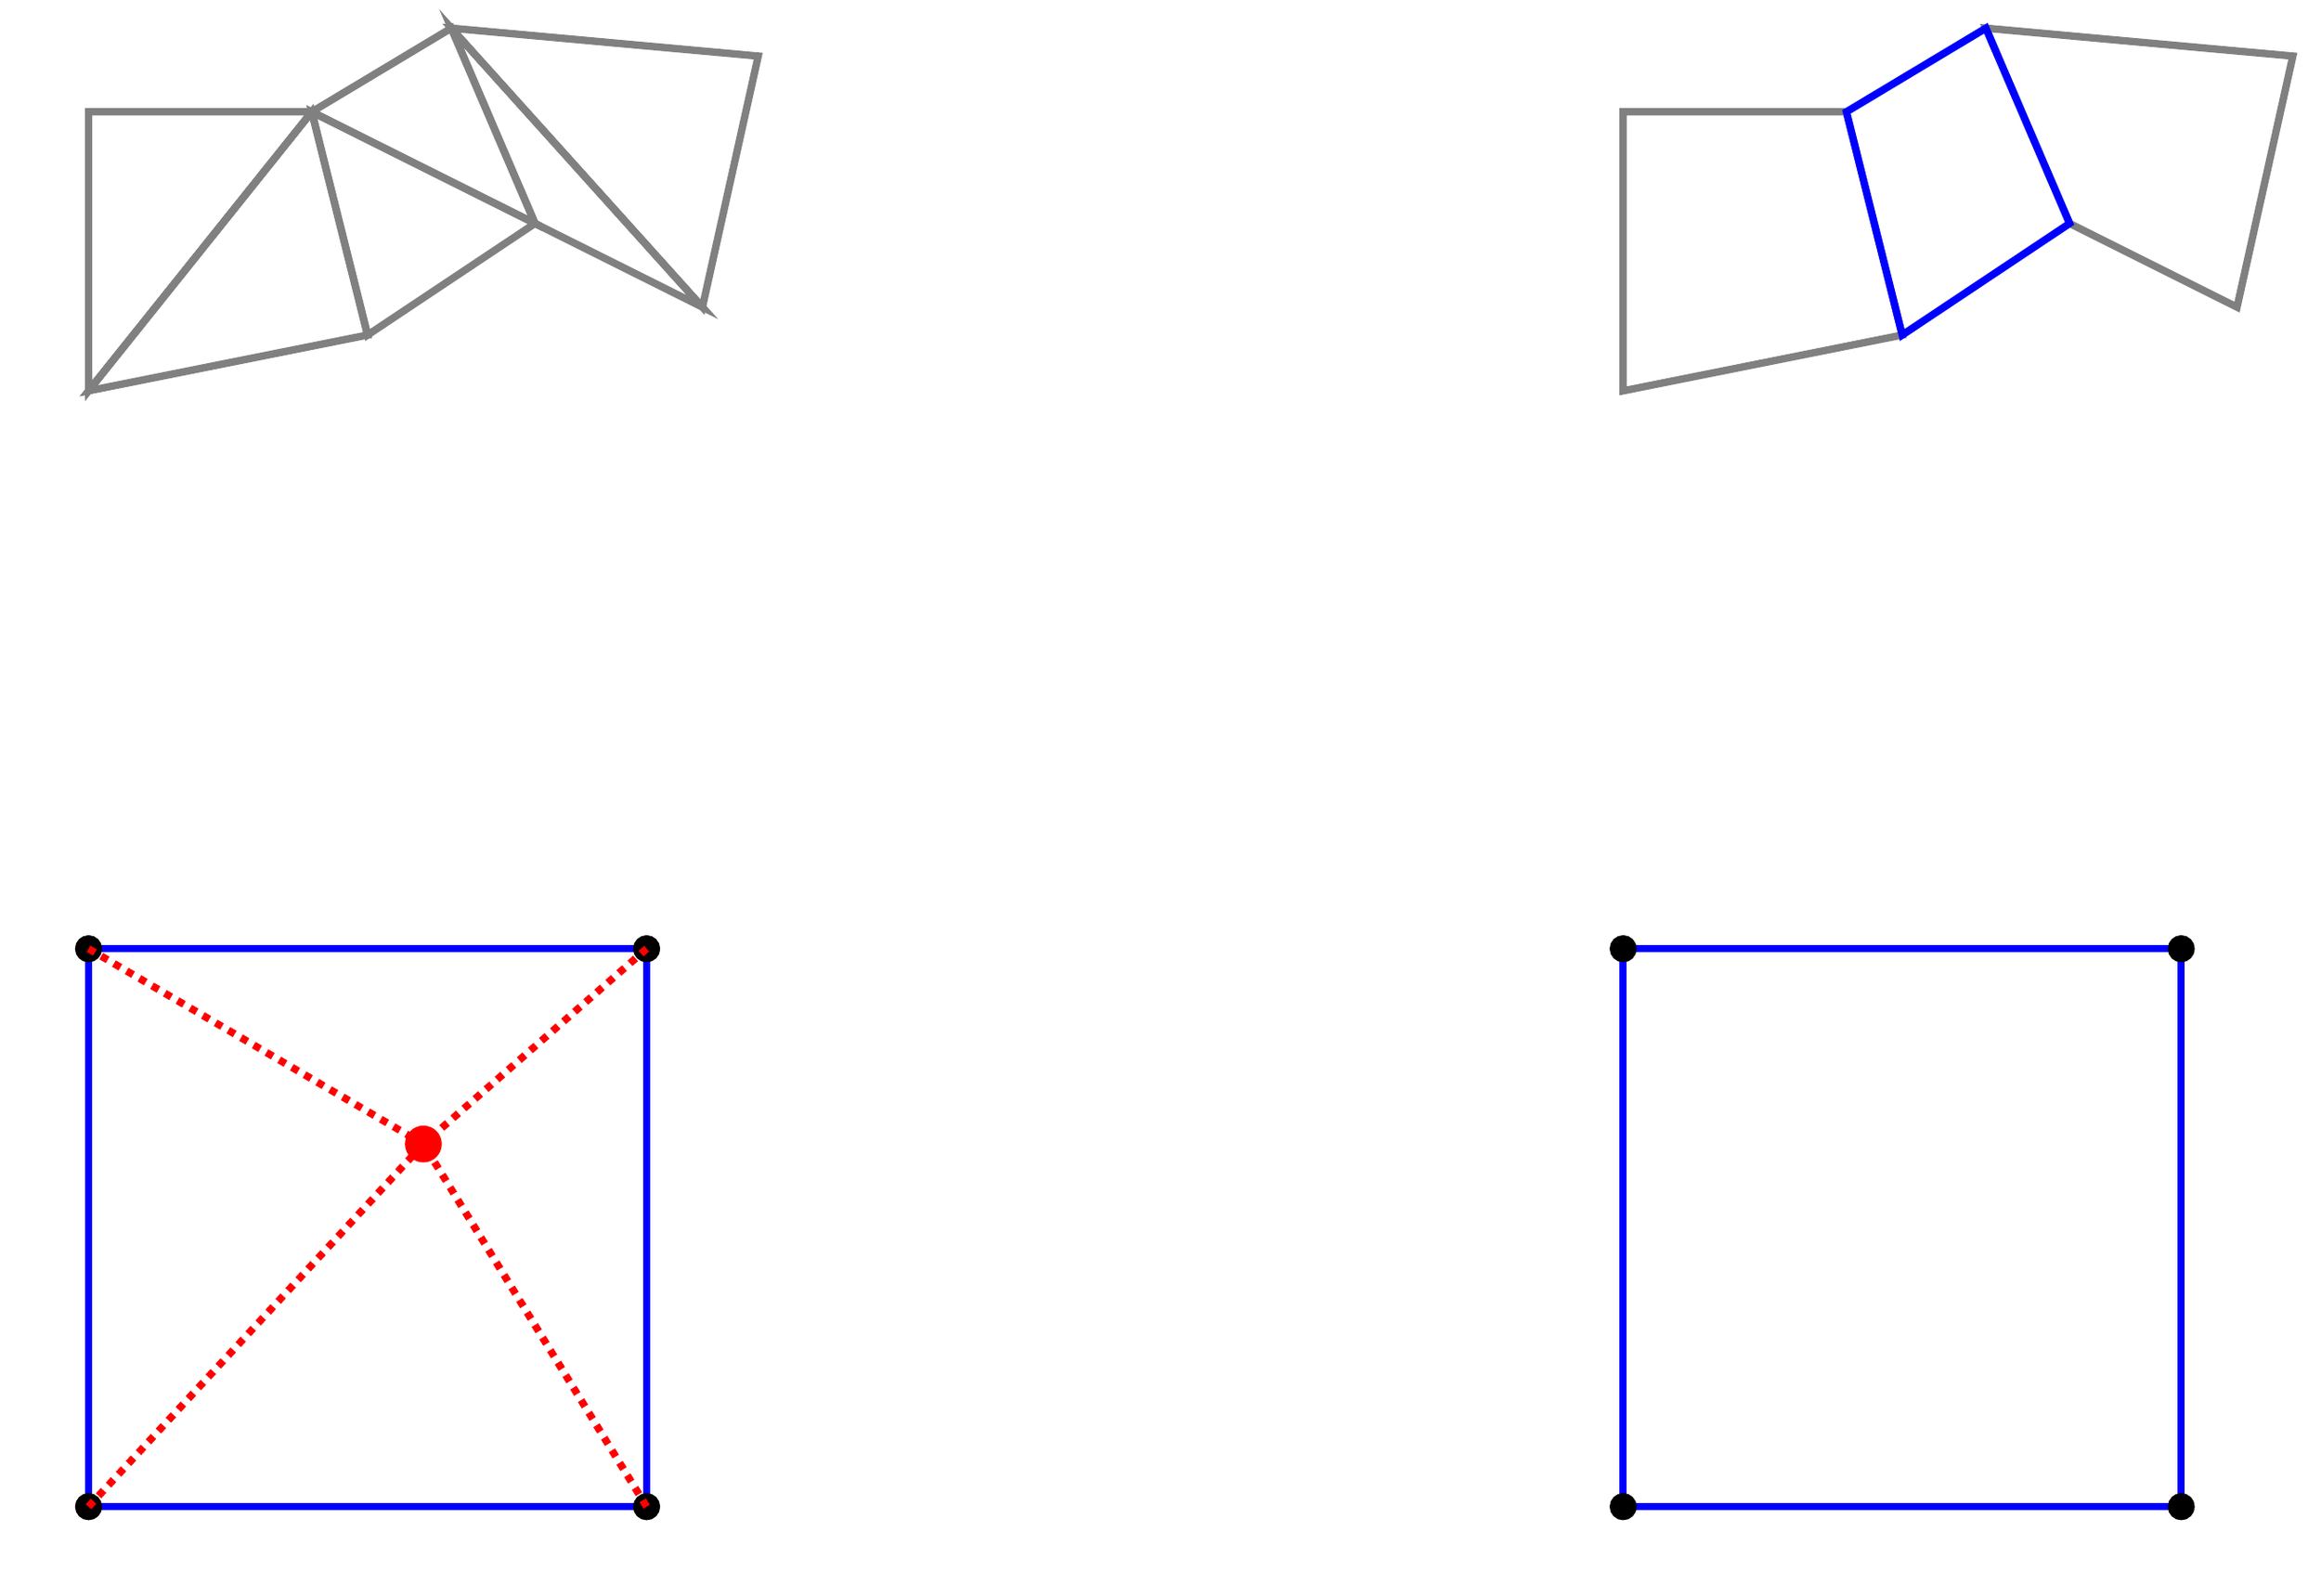
\begin{tikzpicture}[scale=4, every node/.style={scale=0.8}, transform shape,
                    every path/.style={line width=3pt}]  % <-- global line thickness 3pt

  % === Triangle Mesh (Left) ===
  \begin{scope}
    \coordinate (A) at (0,0);
    \coordinate (B) at (1,0.2);
    \coordinate (C) at (0.8,1);
    \coordinate (D) at (0,1);
    \coordinate (E) at (1.6,0.6);
    \coordinate (F) at (1.3,1.3);
    \coordinate (G) at (2.2,0.3);
    \coordinate (H) at (2.4,1.2);

    \draw[gray] (A) -- (B) -- (C) -- cycle;
    \draw[gray] (A) -- (C) -- (D) -- cycle;
    \draw[gray] (B) -- (E) -- (C) -- cycle;
    \draw[gray] (C) -- (E) -- (F) -- cycle;
    \draw[gray] (E) -- (G) -- (F) -- cycle;
    \draw[gray] (F) -- (G) -- (H) -- cycle;
  \end{scope}

  % === Quadrilateral Mesh (Middle) ===
  \begin{scope}[xshift=5.5cm]
    \coordinate (A) at (0,0);
    \coordinate (B) at (1,0.2);
    \coordinate (C) at (0.8,1);
    \coordinate (D) at (0,1);
    \coordinate (E) at (1.6,0.6);
    \coordinate (F) at (1.3,1.3);
    \coordinate (G) at (2.2,0.3);
    \coordinate (H) at (2.4,1.2);

    \draw[gray] (A) -- (B) -- (C) -- (D) -- cycle;
    \draw[gray] (E) -- (G) -- (H) -- (F) -- cycle;
    \draw[blue, line width=3pt] (B) -- (E) -- (F) -- (C) -- cycle; % draw last

  \end{scope}

  % === Unit Square (Right) ===
  \begin{scope}[xshift=5.5cm, yshift=-4.0cm]
    \draw[blue, line width=3pt] (0,0) rectangle (2,2);
    \filldraw[black] (0,0) circle (1pt) node[anchor=north east] {};
    \filldraw[black] (2,0) circle (1pt) node[anchor=north west] {};
    \filldraw[black] (0,2) circle (1pt) node[anchor=south east] {};
    \filldraw[black] (2,2) circle (1pt) node[anchor=south west] {};
  \end{scope}

  % === Feature Field (Left) ===
  \begin{scope}[yshift=-4.0cm]
    \draw[blue, line width=3pt] (0,0) rectangle (2,2);

    % Corner features (bold vectors), with f00 label moved outward
    \filldraw[black] (0,0) circle (1pt) node[anchor=north east] {};
    \filldraw[black] (2,0) circle (1pt) node[anchor=north west] {};
    \filldraw[black] (0,2) circle (1pt) node[anchor=south east] {};
    \filldraw[black] (2,2) circle (1pt) node[anchor=south west] {};

    % Interpolation point (u)
    \filldraw[red] (1.2,1.3) circle (1.5pt) node[right] {};

    % Lines from corners to interpolation point
    \foreach \x/\y in {0/0, 2/0, 0/2, 2/2} {
      \draw[dashed, red] (\x,\y) -- (1.2,1.3);
    }

  \end{scope}

\end{tikzpicture}

\end{document}
